\section{Продолжаем примеры на аксиомы делимости}

\begin{exmpls}
	\item $ X = \R^2 $ \\
    База -- шары с выколотым конечным чилом радиусов \\
    Открытое множество -- множество, такое, что $ \forall x \quad \exist M_x $ указанного вида \\
    $ X $ хаусдорфово, не регулярно
    \item \textbf{Пространство Немыцкого:} \\
    $ X $ -- замкнутая полуплоскость \\
    Открытое множество -- у любой точки существует окрестность специального вида \\
    Окрестности:
    \begin{itemize}
    	\item Если точка не на границе полуплоскости -- окрестность обычного вида (открытый круг)
        \item Если точка на границе полуплоскости -- открытый круг, сдвинутый к краю полуплоскости + сама точка (см. рис. \ref{fig:1})
    \end{itemize}
    $ X $ регулярно, но не нормально
\end{exmpls}

\begin{figure}[!ht]
    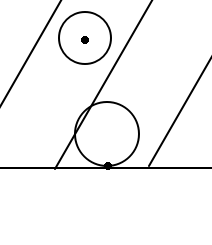
\includegraphics[scale=0.8]{nemyz}
    \caption{Пространство Немыцкого}
    \label{fig:1}
\end{figure}

\section{Нормальные пространства}

\begin{theorem}
	Метрическое простанство нормально
\end{theorem}

\begin{proof}
	\hfill
    \begin{itemize}
    	\item Докажем, что метрическое пространство хаусдорфово: \\
        Для этого надо доказать, что выполняется \textbf{T2}: \\
        Возьмём $ x \ne y, \quad \veps \define \dfrac{\rho(x, y)}2 $
        $$ B(x, \veps) \cap B(y, \veps) = \O $$
        (по неравенству треугольника)
        \item Регулярность:
        $$ x_0 \in X, \quad F \text{ -- замкн. } \implies \exist \rho(x_0, F) \define \inf\limits_{y \in F} \rho(x, y) > 0 \quad ? $$
        Допустим $ \inf\limits_{y \in F}(x_0, y) = 0 $
        \begin{multline*}
            \implies \exist y_n : \rho(x_0, y_n) \underarr{n \to \infty} 0 \implies \forall \veps > 0 \quad \exist N : \forall n > N \quad y_n \in B(x_0, \veps) \implies \\ \implies x_0 \in \Cl\set{y_n} \sub \Cl F = F
        \end{multline*}
        $$ \veps \define \frac{\rho(x_0, F)}2, \qquad U_{x_0} = B(x_0, \veps) $$
        $$ U_F = \bigcup_{y \in F} B(y, \veps) \text{ -- откр.} $$
        \item \textbf{T4} \\
        $ F_1, F_2 $ -- замкнутые, хотим, чтобы $ \rho(F_1, F_2) $ могло равняться нулю
        \begin{eg}
        	$ \R^2 $, обычная топология
        \end{eg}
        $$ \forall x \in F_1 \quad \exist \veps_x \define \frac{\rho(x, F_2)}2 > 0 $$
        $$ \forall y \in F_2 \quad \exist \veps_y \define \frac{\rho(y, F_1)}2 > 0 $$
        Возьмём $ U_{F_1} \define \bigcup_{x \in F_1} B(x, \veps_x), \qquad U_{F_2} \define \bigcup_{y \in F_2} B(y, \veps_y) $
        $$ x \in U_{F_1} \cap U_{F_2} \implies z \in B(x, \veps_x) \cap B(y, \veps_y) $$
        Пусть, НУО, $ \veps_x \ge \veps_y \implies \rho(x, y) < 2\veps_x = \rho(x, F_2) $
        Вспомним, что $ x \in F_1, y \in F_2 $. Получили, что расстояние от $ x $ до некоторой точки фигуры $ F_2 $ больше, чем расстояние до самой $ F_2 $
    \end{itemize}
\end{proof}

\begin{figure}[!ht]
    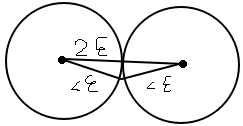
\includegraphics{norm_t2}
    \caption{Доказательство \textbf{T2} для метрического пространства}
\end{figure}

\begin{theorem}
	$ X $ -- компактно и хаусдорфово $ \implies X $ нормально
\end{theorem}

\begin{remark}
	Иногда, ``компакт'' = ``хаусдорфово + компакт''
\end{remark}

\begin{proof}
	\hfill
    \begin{itemize}
    	\item Докажем, что $ X $ регулярно \\
        Возьмём $ x_0 \in X, \quad F $ -- замкн. в $ X $ ($ \implies F $ компактно, в силу хаусдорфовости) \\
        В силу хаусдорфовости,
        $$ \forall y \in F
        \begin{Bmatrix}
            \exist U_{x_0, y} \text{ -- откр.} \\
            \exist V_y \text{ -- откр.}
        \end{Bmatrix} : U_{x_0, y} \cap V_y = \O $$
        Возьмём $ \set{V_y}_{y \in F} $ -- открытое покрытие $ \implies \exist y_1, ..., y_n \in F $ \\
        $ \set{V_{y_i}} $ -- конечное подпокрытие $ F $
        $$ U_{x_0} \define \bigcap_{i = 1}^n U_{x_0, y_i} \text{ -- откр. }, \qquad U_F \define \bigcap_{i = 1}^n V_{y_i} $$
        \item Нормальность: \\
        $ F_1, F_2 $ -- замкнутые непересекающиеся множества \\
        Возьмём $ x \in F_1, \quad \underset{\text{окр. } x}{U_x}, \underset{\text{окр. } F_2}{V_x} : U_x \cap V_x = \O $
        $$ \set{U_x}_{x \in F_1} \text{ -- покр. } F_1 \implies \exist x_1, ..., x_n \in F_1 : \set{U_{x_i}}_{i = 1}^k \text{ -- покр. } F_1 $$
        $$ U_{F_1} \define \bigcup_{i = 1}^n U_{x_i}, \qquad U_{F_2} \define \bigcap_{i = 1}^n V_{x_i} $$
    \end{itemize}
\end{proof}

\section{Компактификация по Александрову (Павлу Сергеевичу)}

\begin{definition}
    $ X $ называется локально компактным, если $ \forall x_0 \in X \quad \exist U_{x_0} : \Cl U_{x_0} $ -- комп. \\
    (у любой точки есть окрестность с компактным замыканием)
\end{definition}

\begin{exmpls}
	\item $ \R^n $ локально компактно
    \item $ \Q $ не локально компактно
\end{exmpls}

\begin{theorem}[Александрова]
    $ X $ локально компактно + хаусдорфово $ \implies \exist \hat{X} \define X \cup \set{\infty}, \quad X $ -- подпространство $ \hat{X} $ \\
    $ \hat{X} $ -- комп. + хаусдорфово
\end{theorem}

\begin{proof}
    По условию, $ \hat{X} = X \cup \set{\infty} $ \\
    Открытые в $ \hat{X} $:
    \begin{itemize}
        \item $ U \not\ni \infty \implies U $ откр. в $ \hat{X} \iff U $ откр. в $ X $
        \item $ U \ni \infty \implies U $ откр. в $ \hat{X} \iff \hat{X} \setminus U (= X \setminus U) $ компактно
    \end{itemize}
    \begin{itemize}
        \item Докажем, что $ X $ -- подпространство $ \hat{X} $: \\
        Нужно доказать, что если $ \infty \in U $, то $ U \setminus \set\infty $ -- откр. в $ X $
        $$ X \setminus \big( U \setminus \set\infty \big) \text{ -- комп. в } X \underimp{X \text{ -- хаусд.}} X \setminus \big( U \setminus \set\infty \big) \text{ -- замкн. } \implies U \setminus \set\infty \text{ -- откр.} $$
        \item Очевидно, что $ X $ компактно
        \item Докажем, что $ X $ хаусдорфово:
        \begin{itemize}
            \item $ x_0, y_0 \in \hat{X} \setminus \set\infty \implies $ ОК (разделяем в $ X $)
            \item $ x_0 \in \hat{X} \setminus \set\infty, y_0 = \infty $:
            $$ \exist U_{x_0} \sub X : \Cl U_{x_0} \text{ -- копм.} $$
            $$ U_{y_0} \define X \setminus \Cl U_{x_0} \text{ -- откр. в } \hat{X} \text{ и \textit{сод.} } y_0 = \infty $$
        \end{itemize}
    \end{itemize}
\end{proof}

\begin{theorem}[Урысона (о функциональной делимости)]
	$ X $ -- норм., $ F_1, F_2 $ -- замкнутые непересекающиеся множества
    $$ \implies \exist \text{ непр. } f : X \to \R :
    \begin{cases}
        f\clamp{F_1} = 0 \\
        f\clamp{F_2} = 1
    \end{cases} $$
\end{theorem}

\begin{proof}
	Без доказательства
\end{proof}

\begin{axiom}[\textbf{T3.5}]
    $ \forall F_1, F_2 $ -- замкн. неперес. $ \quad \exist f : X \to \R \text{ -- непр. }:
    \begin{cases}
    	f\clamp{F_1} = 0 \\
        f\clamp{F_2} = 1
    \end{cases} $
\end{axiom}
